\documentclass[11pt]{article}
\usepackage{verbatim,url,enumerate,color,paralist}
\usepackage{amsmath,amsfonts,amsthm}
\usepackage{epsfig,amssymb,amstext,xspace}\usepackage{algorithm}
\usepackage{algorithmicx,algpseudocode}
\usepackage{fullpage}

\RequirePackage{fix-cm}
\usepackage{graphicx}
\usepackage{subfig}
\usepackage[usenames,dvipsnames]{xcolor}
\usepackage[colorlinks,citecolor=blue,linkcolor=BrickRed]{hyperref}
\usepackage{times}
\usepackage{latexsym,graphicx,epsfig,color,mathdots}
\usepackage{amsfonts,amssymb,amsmath,amstext}
\usepackage{url,setspace}
\usepackage{multirow}
\usepackage{rotating}
\usepackage{tikz}

\usetikzlibrary{decorations.markings}
\usetikzlibrary{arrows}
\tikzstyle{block}=[draw opacity=0.7,line width=1.4cm]
\tikzstyle{graphnode}=[circle, draw, fill=black!20, inner sep=0pt, minimum width=6pt]
\tikzstyle{point}=[circle, draw, fill=black!30, inner sep=0pt, minimum width=1pt]
\tikzstyle{input}=[rectangle, draw, fill=black!75,inner sep=3pt, inner ysep=3pt, minimum width=4pt]
\tikzstyle{unmatched}=[graphnode,fill=black!0]
\tikzstyle{shaded}=[graphnode,fill=black!20]
\tikzstyle{matched}=[graphnode,fill=black!100]  	
\tikzstyle{matching} = [ultra thick]
\tikzset{
>=stealth',
pil/.style={
           ->,
           thick,
           shorten <=2pt,
           shorten >=2pt,}
}
\tikzset{->-/.style={decoration={
  markings,
  mark=at position .5 with {\arrow{>}}},postaction={decorate}}}


\newtheorem{theorem}{Theorem}[section]
\newtheorem{lemma}[theorem]{Lemma}
\newtheorem{corollary}[theorem]{Corollary}
\newtheorem{definition}[theorem]{Definition}
\newtheorem{observation}[theorem]{Observation}
\newtheorem{proposition}[theorem]{Proposition}
\newtheorem{claim}[theorem]{Claim}
\newtheorem{fact}[theorem]{Fact}



\newcommand{\IGNORE}[1]{}

\newcommand{\sa}{\textsf{Sherali-Adams}}
\newcommand{\ls}{\textsf{Lov\'asz-Schrijver}}
\newcommand{\la}{\textsf{Lasserre}}
\newcommand{\lap}{\textrm{Lift-and-Project}}
\newcommand{\iLS}{\textsf{LS}}
\newcommand{\iLSp}{\textsf{LS}}
\newcommand{\iSA}{\textsf{SA}}
\newcommand{\iSAp}{\textsf{SA}}
\newcommand{\pop}{\mathcal{P}}
\newcommand{\iLa}{\textsf{La}}
\newcommand \reals {\mathbb{R}}
\def \integers {\mathbb{Z}}
\newcommand{\xout}[1]{x\left( \delta^{out}(#1)\right)}
\newcommand{\xin}[1]{x\left( \delta^{in}(#1)\right)}
\newcommand{\atspbal}{\homog{\textsf{ATSP}}}
\newcommand{\atspdfj}{\homog{\textsf{ATSP}}}
\newcommand{\atspbalpolytope}{\widehat{\textsf{ATSP}}_{\mathit{BAL}}}
\newcommand{\atspdfjpolytope}{\widehat{\textsf{ATSP}}_{\mathit{DFJ}}}
\newcommand{\PATSP}{\textsf{PATSP}}
\newcommand{\PATSPpolytope}{\widehat{\textsf{PATSP}}}
\newcommand{\tsp}{\textsc{TSP}}
\newcommand{\atsp}{\textsc{ATSP}}
\newcommand{\pathtsp}{\textsc{path~TSP}}
\newcommand{\pathatsp}{\textsc{path~ATSP}}
\renewcommand{\P}{}
\newcommand{\NP}{}
\newcommand\bo {{\bf 0}}
\newcommand\be {{\bf e}}
\newcommand\bu {{\bf u}}
\newcommand\bv {{\bf v}}
\newcommand\bw {{\bf w}}
\newcommand\bx {{\bf x}}
\newcommand\by {{y}}
\newcommand\bz {{z}}
\newcommand{\iLP}{\textsf{LP}}
\newcommand{\iLPs}{\textsf{LP}s}
\newcommand{\gdecomp}[1]{\mathcal{C}(#1)}
\newcommand{\gdecomplong}[2]{\mathcal{C}_{#2}(#1)}
\newcommand{\gdecompsymbol}{\widehat{\mathcal{C}}}
\newcommand{\cindset}{\mathcal{N}}
\newcommand{\fracset}{\mathcal{F}}
\newcommand{\notfracset}{\overline{\mathcal{F}}}
\newcommand{\sgn}{\mathcal{I}}
\newcommand{\yvec}[2]{y^{#1,\,#2}}	\newcommand{\zvec}[2]{y^{#1,\,#2}}	\newcommand{\zveconly}{y}
\newcommand{\onevec}[2]{\textbf{1}^{#1,\,#2}}		\newcommand{\goodfrac}[2]{F^{#1}(#2)}	\newcommand{\szgoodfrac}[2]{f^{#1}(#2)}	\newcommand{\cindex}[1]{\textit{index}(#1)} \newcommand{\indfrac}{h}	\newcommand{\tour}{\textit{tour\/}}
\newcommand{\cone}{\textit{cone\/}}
\newcommand{\opt}{\textit{opt\/}}
\newcommand{\dfj}{\textit{dfj\/}}
\newcommand{\loglog}{\textit{loglog\/}}
\newcommand{\saop}{\mathcal{SA}}
\newcommand{\homog}[1]{{#1}}





\begin{document}

\title{On Integrality Ratios for Asymmetric TSP \\
	in the Sherali-Adams Hierarchy
\footnote{An extended abstract of this work appeared in the proceedings of the 40th International Colloquium on Automata, Languages, and Programming ({ICALP} 2013).}
}


\author{Joseph Cheriyan\thanks{
 Dept. Comb. \& Opt., University of Waterloo, Canada,
 Email:\texttt{jcheriyan,z9gao,k2georgi@uwaterloo.ca}} 
\and Zhihan Gao  
\and Konstantinos Georgiou 
\and
Sahil Singla\thanks{School of Comp.\ Sci., Carnegie Mellon University, USA, 
Email:\texttt{ssingla@cmu.edu}
}
}





\maketitle

\begin{abstract}
We study the \atsp\ (Asymmetric Traveling Salesman Problem), and our
focus is on negative results in the framework of the Sherali-Adams
(\iSA) Lift and Project method.


Our main result pertains to the standard LP (linear programming)
relaxation of \atsp, due to Dantzig, Fulkerson, and Johnson.
For any fixed integer  and small ,
,
there exists a digraph  on

vertices such that the integrality ratio for level~ of the \iSA\ system
starting with the standard LP on  is
.
Thus, in terms of the input size,
the result holds for any  levels.
Our key contribution is to identify
a structural property of digraphs that
allows us to construct fractional feasible solutions
for any level~ of the \iSA\ system starting from the standard~LP.
Our hard instances are simple and satisfy the structural property.

There is a further relaxation of the standard LP called the
balanced LP, and our methods simplify considerably
when the starting LP for the \iSA\ system is the balanced~LP;
in particular, the relevant structural property (of digraphs)
simplifies such that
it is satisfied by the digraphs given by
the well-known construction of Charikar, Goemans and Karloff (CGK).
Consequently, the CGK digraphs serve as hard instances,
and we obtain an integrality ratio of  
for any level~ of the \iSA\ system,
where 
and the number of vertices is
.

Also, our results for the standard~LP extend to the \pathatsp\ (find a
min cost Hamiltonian dipath from a given source vertex to a given sink
vertex).

\paragraph{Keywords:}Asymmetric TSP, Sherali-Adams Hierarchy, Integrality Ratios
\end{abstract}




\section{Introduction}\label{sec:intro}


The Traveling Salesman Problem (\tsp) is a celebrated problem in
combinatorial optimization, with many connections to theory and
practice.  The problem is to find a minimum cost tour of a set of
cities; the tour should visit each city exactly once. The most well
known version of this probelm is the symmetric one (denoted \tsp),
where the distance (a.k.a.~cost) from city~ to city~ is equal to
the distance (cost) from city~ to city~. The more general version
is called the asymmetric TSP (denoted \atsp), and it does not have the symmetry
restriction on the costs. Throughout, we assume that the costs satisfy
the triangle inequalities, i.e., the costs are metric.

Linear programming (LP) relaxations play a central role in solving  \tsp\ 
or \atsp, both in
practice and in the theoretical setting of approximation algorithms.
Many LP relaxations are known for \atsp, see \cite{RT12} for a recent
survey. The most well-known relaxation (and the one that is most useful
for theory and practice) is due to Dantzig, Fulkerson and Johnson; we
call it the standard~LP or the DFJ~LP. It has a constraint for every
nontrivial cut, and has an indegree and an outdegree constraint for
each vertex; see Section~\ref{subsec:atsp-lp}.
There is a further relaxation of the standard~LP that is of interest; we
call it the balanced LP (Bal~LP); it is obtained from the standard~LP
by replacing the indegree and outdegree constraint at each vertex by a
balance (equation) constraint. For metric costs, the optimal value of
the standard~LP is the same as the optimal value of the balanced LP;
this is a well-known fact, see \cite{RT12}, \cite[Footnote~3]{CGK06}.

One key question in the area is the quality of the objective value
computed by the standard~LP.  This is measured by the \textit{integrality
ratio} (a.k.a.~integrality gap) of the relaxation, and is defined to be
the supremum over all instances of the integrality ratio of the
instance.  The integrality ratio of an instance  is given by
, where  denotes the optimum (minimum cost of
a tour) of , and  denotes the optimal value of the standard~LP
relaxation of ; we assume that the optima exist and that
.\footnote{
Although the term integrality ratio is used in two different
senses---one refers to an instance, the other to a relaxation
(i.e., all instances)---the context will resolve the ambiguity.}

For both \tsp\ and \atsp,
significant research efforts have been devoted over several decades
to prove bounds on the integrality ratio of the standard~LP.
For \tsp, methods based on Christofides' algorithm show that
the integrality ratio is ,
whereas the best lower bound known on the integrality ratio is .
Closing this gap is a major open problem in the area.
For \atsp, a recent result of Asadpour et al.~\cite{AGMOS-soda10}
shows that the integrality ratio is .
On the other hand, Charikar, et al.~\cite{CGK06} showed a
lower bound of~2 on the integrality ratio,
thereby refuting an earlier conjecture of Carr and Vempala \cite{CV04}
that the integrality ratio is .

Lampis \cite{lampis12} and Papadimitriou and later Vempala
\cite{papad-vempala-06}, have proved
hardness-of-approximation thresholds of  for \tsp\ and
 for \atsp,  respectively;
both results assume that \P\NP.
Recently, Karpinski, et al \cite{KLS-isaac13} have improved both
hardness-of-approximation thresholds to
123/122 and 75/74, respectively, assuming that \P\NP.


Our goal is to prove lower bounds on the integrality ratios for \atsp\ 
for the tighter LP relaxations obtained by applying
the Sherali-Adams Lift-and-Project method.
Before stating our results, we present an overview of Lift-and-Project
methods.


\subsection{Hierarchies of convex relaxations}


Over the past 25 years, several methods have been developed in order
to obtain tightenings of relaxations in a systematic manner.
Assume that each variable  is in the interval ,
i.e., the integral solutions are zero/one, and
let  denote the number of variables in the original relaxation.
The goal is to start with a simple relaxation,
and then iteratively obtain a sequence of
stronger/tighter relaxations
such that the associated polytopes form a nested family
that contains (and converges to) the integral hull\footnote{
By the \textit{integral hull} we mean
the convex hull of the zero-one solutions
that are feasible for the original relaxation.}.


These procedures, usually called {\em Lift-and-Project}
hierarchies (or systems, or methods, or procedures),
use polynomial reasonings together with
the fact that in the 0/1 domain, general polynomials can be reduced
to multilinear polynomials (utilizing the identity ), and
then finally obtain a stronger relaxation by applying linearization
(e.g., for subsets  of ,
the term  is replaced by a variable ).
In this overview, we gloss over the Project step.
In particular,
Sherali and Adams~\cite{SA90} devised the \sa\ (\iSA) system,
Lov\'asz and Schrijver~\cite{LS91}
devised the \ls\ (\iLS) system,
and Lasserre~\cite{las02} devised the \la\ system.
See Laurent~\cite{Lau03} for a survey of these systems;
several other Lift-and-Project systems are known,
see~\cite{CM-chapter,AT-ipco11}.


The index of each relaxation in the sequence of tightened relaxations
is known as the \textit{level} in the hierarchy; the level of the
original relaxation is defined to be zero.
For each of these hierarchies and for any ,
it is known that
the relaxation at level  of
the hierarchy can be solved to optimality in polynomial time,
assuming that the original relaxation has
a polynomial-time separation oracle,
\cite{tourlakisthesis06}
(additional mild conditions may be needed for some hierarchies).
In fact, the relaxation at level  is exact, i.e.,
the associated polytope is equal to the integral hull.


Over the last two decades,
a number of important improvements on approximation guarantees have
been achieved based on relaxations obtained from Lift-and-Project
systems.
See \cite{CM-chapter} for a recent survey of many such positive results.


Starting with the work of Arora et al.~\cite{ABLT06},
substantial research efforts have been devoted to
showing that tightened relaxations (for many levels) fail to reduce
the integrality ratio for many combinatorial optimization problems
(see~\cite{CM-chapter} for a list of negative results).
This task seems especially difficult for
the \iSA\ system because it strengthens
relaxations in a ``global manner;''
this enhances its algorithmic leverage for deriving positive results,
but makes it more challenging
to design instances with bad integrality~ratios.
Moreover, an integrality ratio for the \iSA\ system may be viewed as an
unconditional inapproximability result for a restricted model of
computation, whereas, hardness-of-approximation results are usually
proved under some complexity assumptions, such as {\P}{\NP}.
The \iSA\ system is known to be more powerful than
the \iLS\ system, while it is weaker than the \la\ system;
it is incomparable with the \iLSp\ system
(the positive-semidefinite version of the \ls\ system \cite{LS91}).



A key paper by Fern\'andez de la Vega and Kenyon-Mathieu \cite{FK07}
introduced a probabilistic interpretation of the \iSA\ system, and
based on this, negative results (for the \iSA\ system) have been proved
for a number of combinatorial problems;
also see
Charikar et al.~\cite{CMM09}, and Benabbas, et al.~\cite{BCGM11}.
At the moment, it is not clear that methods based on \cite{FK07} could
give negative results for \tsp\ and its variants, because the natural
LP relaxations (of \tsp\ and related problems) have ``global
constraints.''




To the best of our knowledge, there are only two previous papers with
negative results for Lift-and-Project methods applied to \tsp\ and its
variants.
Cheung~\cite{cheung05} proves an integrality ratio of
 for \tsp, for  levels of \iLSp.
For \atsp, Watson~\cite{watson11} proves an integrality ratio of
 for level~1 of the \ls\ hieararchy, starting from the
balanced~LP (in fact, both the hierarchies \iLS\ and \iSA\ give the
same relaxation at level~one).

We mention that Cheung's results~\cite{cheung05}
for \tsp\ do not apply to \atsp, although
at level~0, it is well known that
any integrality ratio for the standard~LP for \tsp\
applies also to the standard~LP for \atsp\ 
(this relationship does not hold for level~1 or higher).



\subsection{Our results and their significance}


Our main contribution
is a generic construction of
fractional feasible solutions
for any level~ of the \iSA\ system starting from
the standard~LP relaxation of \atsp.
We have a similar but considerably simpler construction
when the starting LP for the \iSA\ system
is the balanced~LP.
Our results on integrality ratios are direct corollaries.


We have the following results pertaining to
the balanced~LP relaxation of \atsp:
We formulate a property of digraphs that we call
the good decomposition property, and
given any digraph with this property,
we construct a vector  on the edges such that
 is a fractional feasible solution to
the level~ tightening of the balanced~LP by the \sa\ system.
Charikar, Goemans, and Karloff (CGK) \cite{CGK06}
constructed a family of digraphs for which
the balanced~LP has an integrality ratio of~2.
We show that the digraphs in the CGK family
have the good decomposition property,
hence, we obtain an integrality ratio for level~ of \iSA.
In more detail,
we prove that for any integer  and small enough ,
there is a digraph  from the CGK family
on 
vertices such that the integrality ratio of the level- tightening of
Bal LP is at least
 (where  identifies the original relaxation). 


Our main result pertains to the standard~LP relaxation of \atsp.
Our key contribution is to identify
a structural property of digraphs that
allows us to construct fractional feasible solutions
for the level~ tightening of the standard~LP by the \sa\ system.
This construction is much more difficult than the
construction for the balanced~LP.
We present a simple family of digraphs that
satisfy the structural property, and this immediately
gives our results on integrality ratios.
We prove that for any integer  and small enough ,
there are digraphs  on  vertices
such that the integrality ratio of
the level~ tightening of the standard~LP on 
is at least .
The \textit{rank} of a starting relaxation (or polytope)
is defined to be the minimum number of tightenings
required to find the integral hull (in the worst case).
An immediate corollary is that
the \iSA-rank of the standard~LP relaxation on a digraph 
is at least linear in , whereas,
the rank in terms of the number of edges is 
(since the LP is on a complete digraph, namely, the metric completion).

Our results for the balanced~LP and for the standard~LP
are incomparable, because
the \iSA\ system starting from the standard~LP
is strictly stronger than
the \iSA\ system starting from the balanced~LP,
although both the level~zero LPs have the
same optimal value, assuming metric costs.
(In fact, there is an example on 5~vertices
\cite[Figure~4.4,~p.60]{paulthesis08} such that
the optimal values of the level~1 tightenings are different:
 for the balanced~LP and  for the standard~LP.)

Finally, we extend our main results to the natural relaxation of
\pathatsp\ (min cost Hamiltonian dipath from a given source vertex to a
given sink vertex), and
we obtain integrality ratios  for the level-
\iSA\ tightenings.
Our result on \pathatsp\ is obtained by ``reducing'' from the result
for \atsp; the idea behind this comes from an analogous result of
Watson \cite{watson11} in the symmetric setting; Watson gives a method
for transforming Cheung's \cite{cheung05} result on the integrality
ratio for \tsp\ to obtain a lower bound on the integrality ratio for
\pathtsp.


The solutions given by our constructions are \textit{not}
positive semidefinite;
thus, they do not apply to the \iLSp\ hierarchy
nor to the \la\ hierarchy.

Let us assess our results, and place them in context.
Observe that our integrality ratios fade out as the
level of the \iSA\ tightening increases,
and for  (roughly)
our integrality ratio falls below the hardness~threshold of
 of \cite{KLS-isaac13}.
Thus, our integrality ratios cannot be optimal, and it is possible
that an integrality ratio of~2 can be proved for  levels
of the \iSA\ system.

On the other hand,  our results are not restricted to .
For example, parameterized with respect to the number of vertices in
the input , our lower bound for the standard~LP holds even for
level~, and our lower bound for the balanced~LP
(which improves on our lower bound for the standard~LP)
holds even for level~, thus giving
unconditional inapproximability results for these restricted
algorithms, even allowing super-polynomial running time.

Moreover, our results (and the fact that they are not optimal)
should be contrasted with the
known integrality~ratio results for the level~zero standard~LP,
a topic that has been studied for decades.














\section{Preliminaries}

When discussing a digraph (directed graph), we
use the terms dicycle (directed cycle), etc.,
but we use the term edge rather than directed edge or arc.
For a digraph  and ,
 denotes ,
the set of edges outgoing from ,
and  denotes .
For  and ,
 denotes .

By the \textit{metric completion} of a
digraph  with nonnegative edge costs ,
we mean the complete digraph  on 
with the edge costs ,
where  is taken to be the minimum cost (w.r.t. )
of a  dipath of .


An \textit{Eulerian subdigraph} of  is defined as follows:
the vertex set is 
and the edge set is a ``multi-subset'' of 
(that is, each edge in  occurs zero or more times)
such that (i) the indegree of every vertex equals its outdegree, and
(ii) the subdigraph is weakly connected (i.e., the underlying
undirected graph is connected). The ATSP on the metric completion 
of  is equivalent to finding a minimum cost Eulerian subdigraph of
.


For a positive integer  and a ground set , let  denote the
family of subsets of  of size at most , i.e.,
.
We usually take the ground set to be the set of edges of a fixed digraph.
Now, let  be a digraph, and
let the ground set (for ) be .
Let  be a subset of .
Let  denote a vector indexed by elements of 
such that for any ,  if ,
and , otherwise.
Note that  has the entry for  at 1,
and the other entries give the incidence vector of .


We denote set difference by , and
we denote the addition (removal) of a single item 
to (from) a set  by  (respectively, ),
rather than by  (respectively, ).


\subsection{LP relaxations for Asymmetric \tsp}\label{sec:atsp-relaxations}
\label{subsec:atsp-lp}

Let  be a digraph with nonnegative edge costs . Let
 be the feasible region (polytope) of the following
linear program that has a variable  for each edge  of :

In particular, when  is a complete digraph with metric costs, the
above linear program is the standard~LP relaxation of ATSP
(a.k.a.~DFJ~LP).

We obtain the balanced~LP (Bal~LP) from the standard~LP by
replacing the two constraints

by the constraint
,
for each vertex .
Let  be the feasible region (polytope) of Bal~LP.

In particular, when  is a complete digraph with metric costs, the
above linear program is the balanced~LP relaxation of ATSP.

Our construction of fractional feasible solutions exploits the
structure of the original digraph.
This is the reason for discussing the polytopes on the original digraph
(and not only on the complete digraph).
To justify this, we observe that any feasible solution for the original
digraph can be extended to a feasible solution for the complete digraph
by ``padding with zeros.'' (This argument is formalized in Section
\ref{sec:EVto0}).





\subsection{The \sa\ system}

\begin{definition}[The \sa\ system]\label{def:SA-definition}
Consider a polytope  over the variables
, and its description by a system of linear
constraints of the form ;
note that the constraints  and 
for all 
are included in the system.
The level- \sa\ tightened relaxation 
of , is an \iLP\ over the variables
 
(thus,  where
 has ground~set );
moreover, we have .
For every constraint 
of  and for every disjoint 
with , the following is a constraint of the
level- \sa\ relaxation.

\end{definition}


We will use a convenient abbreviation:
  
where  are auxiliary variables between 0 and 1. 

Informally speaking, the level- \sa\ relaxation is derived by
multiplying any constraint of the original relaxation by the high
degree polynomial 

where
 are disjoint subsets of  with .
After expanding the products, we obtain a polynomial of degree at most
. Replacing any occurrences of  by the
corresponding variable  for all  gives
the constraint described in Inequality~\eqref{equa:sa-constraint}
(Definition~\ref{def:SA-definition}).


There are a number of approaches for certifying that  for a given . One popular approach is to give a
probabilistic interpretation to the entries of , satisfying
certain conditions. We follow an alternative approach, that is
standard, see \cite{Lau03}, \cite[Lemma~2.9]{tourlakisthesis06},
but has been rarely used in the context of integrality ratios.

First, we introduce some notation.
Given a polytope ,
consider the cone
.
(Throughout the paper, we use an accented symbol to denote a polytope,
e.g., , and
the symbol (without accent) to denote the associated cone, e.g., .)
It is not difficult to see
that the \iSA\ system can be applied to the cone , so that
the projection in the  original variables
can be obtained by projecting
any  with 
on the  original variables.
Note that  is a cone, hence,
we may have  with ;
but if ,
we can replace  by .
Also, note that  by Definition~\ref{def:SA-definition}.

For a vector  indexed by subsets of  of size at
most , define a \textit{shift operator} ``'' as follows:
for every , let  to be a vector indexed by
subsets of  of size at most , such that .
We have the following folklore fact, \cite[Lemma~2.9]{tourlakisthesis06}.

\begin{fact}.~ \label{fact:recursive-SA}
.
\end{fact}


The reader familiar with the \ls\ system may recognize the similarity
of its definition with the characterization of the \sa\ system of
Fact~\ref{fact:recursive-SA}. In fact, the \iSA\ system differs from
the \iLS\ system only in that it imposes additional consistency
conditions; namely, the moment vector , indexed by subsets of size
, has to be fixed beforehand.
This seemingly small detail gives the \iSA\ system enhanced power
compared to the \iLS\ system.


\subsubsection{Eliminating Variables to 0}\label{sec:EVto0}

In our discussion of the standard~LP and the balanced~LP,
it will be convenient to restrict
the support to the edge set of a given digraph
rather than the complete digraph.
Thus, we assume that some of the variables are absent.
Formally, this is equivalent to setting
these variables in advance to zero.
As long as the nonzero variables induce a feasible solution, we are
justified in setting the other variables to zero.
The following result formalizes the arguments.

\begin{proposition}
Let  be the feasible region (polytope) of a linear program.
Let  be a set of indices (of the variables) that does not contain
the support of any ``positive constraint'' of , where a
constraint  of  is called
positive if .
Let  be the feasible region (polytope) of the linear
program obtained by removing all variables with indices in  from the
constraints of the linear program of  (informally, the
new LP fixes all variables with indices in  at zero).
Then, for the \iSA\ system,
for any feasible solution  to the level- tightening of
, there exists a feasible solution  to the
level- tightening of ; moreover,  is obtained from
 by fixing variables,
indexed by subsets intersecting , to zero.
\end{proposition}
\begin{proof}
For , the ``extension''  of
 is defined as follows:

For the corresponding auxiliary variables , this would imply that

In order to show that , we need to
verify that for every pair of sets  as in
Definition~\ref{def:SA-definition}, we have
.

First we note that if , then for every
 we have , and hence the
constraint is satisfied trivially.

For the remaining case , we have

where~\eqref{equa:feasibility-smaller-polytope} follows from the
validity of the corresponding constraint of ;
here, we use the fact that  does not contain the support of any
positive constraint -- otherwise, the summation 
would be zero since the index set  would be empty,
and hence, the inequality

would fail to hold for  and .
\end{proof}







\section{\iSA\ applied to the Balanced~LP relaxation of ATSP}
\subsection{Certifying a feasible solution} \label{section:balanced}

\begin{figure}[htb]
{
\centerline{
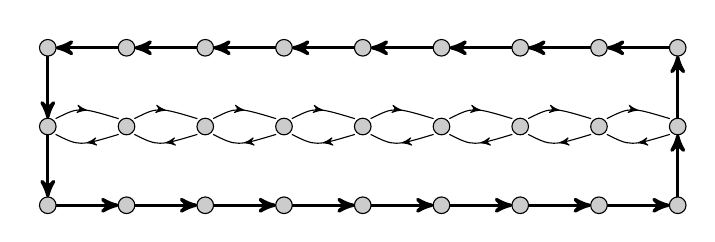
\begin{tikzpicture}[thin,scale=1.0]
\foreach \x in {0,1,2,...,8}
{
	\node at (\x , 0) [graphnode]{};
	\node at (\x , 1) [graphnode]{};
	\node at (\x , 2) [graphnode]{};
}
\foreach \x in {0,1,2,...,7}
{
	\draw [->, very thick] (\x +0.1 , 0) to node[auto]{} (\x + 1-0.1 , 0);
	\draw [<-, very thick] (\x +0.1, 2) to node[auto]{} (\x + 1-0.1 , 2);
}
\foreach \y in {0,1}
{
	\draw [<-, very thick] (0 , \y +0.1) to node[auto]{} (0 , \y +1-0.1);
	\draw [->, very thick] (8 , \y +0.1) to node[auto]{} (8 , \y +1-0.1);
}
\foreach \x in {0,1,2,...,7}
{
	\draw [->-] (\x +0.1 , 1+0.1) .. controls(\x + 0.4, 1.25) .. node[auto]{} (\x + 1-0.1 , 1+0.1);
	\draw [->-] (\x + 1-0.1 , 1-0.1) .. controls(\x + 0.4, 0.75) .. node[auto]{} (\x +0.1 , 1-0.1);
}
\end{tikzpicture}
}
\caption{ A digraph  with a good decomposition given by the dicycle
with thick edges, and the length~2 dicycles  formed by the
anti-parallel pairs of thin edges;  is strongly connected
for each dicycle .}
\label{fig-bal}
}
\end{figure}


A strongly connected digraph  is said to have
a \textit{good~decomposition} with
\textit{witness~set} 
if the following hold
\begin{itemize}
\item[(i)]
 partitions into edge-disjoint dicycles ,
that is, there exist edge-disjoint dicycles 
such that ;
let  denote the set of indices of these dicycles, thus
;
\item[(ii)]
moreover, there exists a nonempty subset  of 
such that for each 
the digraph  is strongly connected.
\end{itemize}

Let  denote .
For an edge , we use  to denote the index  of the
dicycle  that contains .
In this section, by a dicycle  etc.,
we mean one of the dicycles , and
we identify a dicycle  with its edge set, .
See Figure~\ref{fig-bal} for an illustration
of a good decomposition of a digraph.

Informally speaking, our plan is as follows:
for digraph  that has a good decomposition with witness set ,
we construct a feasible solution to 
by assigning the same fractional value to the edges of
the dicycles  with ,
while assigning the value 
to the edges of the dicycles  with 
(this is not completely correct; we will refine this plan).
Let  be the associated cone of .




\begin{definition}
\label{def:goodfrac}
Let  be a nonnegative integer.
For any set  of size , and
any subset  of ,
let  denote
the set of indices  such that
;
moreover, let  denote ,
namely, the number of dicycles  with indices in 
that intersect .
\end{definition}


\begin{definition}
\label{def:balanced}
For a nonnegative integer  and
for any subset  of ,
let  be a vector indexed by the elements of
 and defined as follows:

\end{definition}

\begin{theorem}
\label{thm:balanced}
Let  be a strongly connected digraph that
has a good decomposition,
and let  be the witness~set. Then

\end{theorem}
In order to prove our integrality ratio result for , we will invoke Theorem~\ref{thm:balanced} for  (the more general setting of the theorem is essential for our induction proof; we give a high-level explanation in the last paragraph of the proof of Theorem~\ref{thm:balanced} below). 
Since also only the values of  indexed at singleton edges affect the integrality ratio, 
it is worthwhile to summarize all relevant quantities in the next corollary. 


\begin{corollary}
\label{coro:balanced-empty}
We have

Moreover, 
for each dicycle , , and each edge  of  we have

\end{corollary}


Informally speaking, we assign the value~1
(rather than a fractional value) to the edges of
the dicycles  with .
For the sake of exposition,
we call the dicycles  with 
the \emph{fractional dicycles}, and
we call the remaining dicycles 
(thus ) the \emph{integral dicycles}.

\begin{proof}[Proof of Theorem \ref{thm:balanced}:~]
To prove Theorem \ref{thm:balanced}, we need to prove

We prove this by induction on .

Note that  by Definition \ref{def:balanced}.

The induction basis is important, and it follows easily from the
good decomposition property.
In Lemma~\ref{lemma:base} (below) we show that
. 
We conclude that  satisfies the first two sets of constraints of 
, since 
(this follows from Definitions~\ref{def:goodfrac},\ref{def:balanced}, since
). As for the balance constraints, it is enough to observe that every vertex of our instance (see Figure~\ref{fig-bal}) is incident to pairs of outgoing and ingoing edges, which due to Definition~\ref{def:balanced} are assigned the same value. Finally, again by Definition~\ref{def:balanced}, and for all edges , we have . All the above imply that , as wanted. 

In the induction step, we assume that
 for some integer 
(the induction hypothesis),
and we apply the recursive definition based
on the shift operator,
namely,
 iff for each 

Lemma~\ref{lemma:cond1} (below) proves (\ref{eq:cond1}) and
Lemma~\ref{lemma:cond2} (below) proves (\ref{eq:cond2}).
\end{proof}

We prove that  is in 
by showing that for some edges ,
 is a scalar multiple of  ,
where 
(see Equation~\eqref{eqn:bal-case1} in Lemma~\ref{lemma:cond1});
thus, the induction hinges on the use of .


Before proving Lemma~\ref{lemma:cond1} and Lemma~\ref{lemma:cond2},
we show that , restricted to ,
can be written as a convex combination
of  and the integral feasible solution .
This is used in the proof of Lemma~\ref{lemma:cond1};
for some of the edges ,
we show that 
(see Equation~\eqref{eqn:bal-case1}),
and then we have to show that the latter is in .


\begin{fact}.~ \label{fact:recursive}
Let  be a nonnegative integer and let  be a subset of .
Then for any  we have \qquad

\end{fact}
\begin{proof}
We have , , and
we get  from the definition. Thus,

\end{proof}


\begin{lemma}
\label{lemma:cond1}
Suppose that ,
for each .
Then for all  and for all  we have

\end{lemma}
\begin{proof}
For any , the definition of the shift operator gives

Let  denote the dicycle containing edge , and recall
that  denotes the index of .

We first show that

If , that is, the dicycle 
is not ``fractional,'' then Definition~\ref{def:balanced} directly
gives .
Otherwise, if , then
from Definition~\ref{def:balanced} we see that
if , then
,
and otherwise,
.
Hence,


where in the last line we use Definition~\ref{def:balanced} to infer
that
 , if
, and
 , otherwise.

Note that Fact~\ref{fact:recursive} along with  implies that
, restricted to ,
is in  because
it can be written as a convex combination of  and an
integral feasible solution .
Equation~\eqref{eqn:bal-case1} proves Lemma \ref{lemma:cond1} because
both  and
 (restricted to ) are in
.
 \end{proof}


\begin{lemma}
\label{lemma:cond2}
Suppose that ,
for each .
Then for all  and for all  we have
.
\end{lemma}

\begin{proof}
Let  denote the dicycle containing edge , and recall
that  denotes the index of .
If ,
then we have ,
hence, we have , and
the lemma follows.

Otherwise, we have .
Then, for any , Equation~\eqref{eqn:shift} gives

The good-decomposition property of  implies that
 is
a feasible integral solution of \\ .
\end{proof}


\begin{lemma}
\label{lemma:base}
We have \qquad

\end{lemma}
\begin{proof}
Observe that  has  elements,
and 
(by Definition~\ref{def:balanced});
the other  elements are indexed by
the singleton sets of .
For notational convenience, let  denote
the restriction of  to
indices that are singleton sets;
thus, .
By Definition~\ref{def:balanced},
 if  where ,
and , otherwise.
We claim that  is a feasible solution to .

 is clearly in .
Moreover,  satisfies the balance-constraint at each vertex because it
assigns the same value (either  or 1) to every edge in a dicycle
, .


To show feasibility of the cut-constraints, consider any cut . Since  is a feasible solution, there
exists an edge  crossing from  to . If , then we have , which implies

(from the balance-constraints at the vertices).
 Otherwise, we have .
Applying the good-decomposition property of ,
we see that there exists an edge
 such that , i.e., . Since  for each , the  cut-constraints
 are satisfied.
\end{proof}

The next result presents our first lower bound on the integrality ratio for
the level~ relaxation of the \sa\ procedure starting with the balanced~LP.
The relevant instance is a simple digraph on  vertices;
see Figure~\ref{fig-bal}.
In the next subsection, we present better integrality ratios
using the CGK construction,
but the CGK digraph is not as simple and it has  vertices.

\begin{theorem}\label{thm:sgbalIR}
Let  be a nonnegative integer, and let 
satisfy .
There exists a digraph on  vertices
such that the integrality ratio for
the level~ tightening of the balanced~LP (Bal~LP)
(by the \sa\ system)
is .
\end{theorem}

\begin{proof}
Let  be the digraph together with the good~decomposition shown
in Figure~\ref{fig-bal}, and
let the cost of each edge in  be .
We call an edge of  a \emph{thin} edge if it is contained
in a dicycle of length~2;
we call the other edges of  the \emph{thick} edges;
see the illustration in Figure~\ref{fig-bal}.
Consider the metric completion  of .
It can be seen that the optimal value of
an integral solution of ATSP on 
(equivalent to the minimum cost Eulerian subdigraph of )
is ,
where  is the length of the ``middle path.''
(This can be proved by induction on , using similar arguments as
in Cheung~\cite[Claim~3~of~Theorem~11]{cheung05}.)

Given  and , we
fix  to get a digraph 
(and its edge costs) from the above family.

By Corollary~\ref{coro:balanced-empty}
the fractional solution 
(Definition \ref{def:balanced})
is in :
we have
 for each thick edge , and
 for each thin edge .
By Section \ref{sec:EVto0}, we can extend  to a
feasible solution of .

Hence, the integrality ratio is

\end{proof}






\subsection{CGK (Charikar-Goemans-Karloff) construction}

We briefly explain the CGK~\cite{CGK06} construction and show in
Theorem~\ref{thm:CGK} that the resulting digraph has a good
decomposition. This theorem along with a lemma from \cite{CGK06}
shows that the integrality ratio is 
for  rounds of the \sa\ procedure
starting with the Balanced~LP,
for any given , see Theorem~\ref{thm:IR-CGK}.


Let  be a fixed positive integer.
Let  be the digraph with a single vertex.
Let  consist of a bidirected path
of  vertices, starting at the ``source''  and ending
at the ``sink'' , whose  edges have cost  (see
Figure~\ref{fig:G1}).
We call  the \textit{external} edge~set of 
(we use this in the proof of Lemma~\ref{lem:pre_CGK}).


{
\begin{figure}[h!]
\centering
\subfloat[]{
\begin{tikzpicture}
        \node at (0 , 0) [graphnode]{};
        \node at (2,0)[]{};
        \node at (-2,0)[]{};
\end{tikzpicture}
}
\subfloat[]{
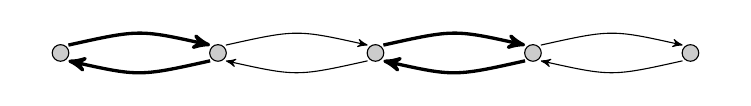
\begin{tikzpicture}
\foreach \x in {0,1,2,3,4}
{
        \node at (2*\x , 0) [graphnode]{};
}
\foreach \x in {1,2,3,4}
{
\node at (2*\x -1,0 )[]{ };
}

\node at (0-0.3 , 0) []{ };
\node at (8+0.3 , 0) []{ };

\foreach \x in {0,2}
{
        \draw [->,very thick] (2*\x +0.1 , 0.1) .. controls (2*\x +1,0.3) ..
(2*\x + 2-0.1 , 0.1);
        \draw [<-,very thick] (2*\x +0.1 , -0.1) .. controls (2*\x +1,-0.3)
.. (2*\x + 2-0.1 , -0.1);
}
\foreach \x in {1,3}
{
        \draw [->] (2*\x +0.1 , 0.1) .. controls (2*\x +1,0.3) .. (2*\x + 2-0.1 , 0.1);
        \draw [<-] (2*\x +0.1 , -0.1) .. controls (2*\x +1,-0.3) .. (2*\x +
2-0.1 , -0.1);
}
\end{tikzpicture}
}
\caption{ and  for }
\label{fig:G1}
\end{figure}

\begin{figure}[h]
\centering
\usetikzlibrary{shapes,snakes}
\tikzstyle{grapheps}=[ellipse, minimum height=.6cm,minimum
width=3.5cm,draw,fill=black!10]
\begin{tikzpicture}[thin,scale=0.8]
\foreach \z in {1,2,3}
{
        \node at (-2 + 5*\z -5, 8.5) [] {};
        \node at (-2 + 5*\z -5, -0.5) [] {};
}
        \draw  [dash pattern=on5pt][->-, very thick] (8 , 8) .. controls (3 ,
10) .. (-2 , 8);
        \draw  [dash pattern=on5pt][->-, very thick] (-2 , 0) .. controls (3
, -2) .. (8 , 0);

\foreach \z in {1,2,3}
{
        \foreach \x in {1,2,...,3}
        {
                \node at (-7 +5*\z, -2*\x + 8) [grapheps]{};
                \node at (-7 +5*\z, -2*\x + 8) []{};
        }
}

\foreach \z in {0,5,10}
{
        \foreach \x in {1,2,...,3}
        {
                \foreach \y in {0,4}
                {
                        \node at (-\y +\z, 2*\x) [graphnode]{};
                }
        }


        \node at (-2 +\z, 0) [graphnode]{};
        \node at (-2 +\z, 8) [graphnode]{};

        \foreach \x in {1,2}
        {
                \ifthenelse{\z =0 \OR \z= 10}
                {
                        \draw [->-] (0 +\z, 2*\x +0.1 ) to  (0 +\z, 2*\x + 2-0.1 );
                        \draw [->-,very thick]  (-4 +\z, 2*\x + 2-0.1) to (-4 +\z, 2*\x +0.1 );
                }
                {
                        \draw [->-,very thick] (0 +\z, 2*\x +0.1 ) to  (0 +\z, 2*\x + 2-0.1 );
                        \draw [->-]  (-4 +\z, 2*\x + 2-0.1) to (-4 +\z, 2*\x +0.1 );
                }
        }
        \ifthenelse{\z =0 \OR \z= 10}
        {
                \draw [->-,very thick] (-4 +\z, 2) to (-2 +\z, 0) node[pos=0.5,below] {};
                \draw [->-,very thick] (-2 +\z, 8) to (-4 +\z, 6) node[pos=0.5,below] {};
                \draw [->-] (-2 +\z, 0) to (0 +\z, 2*0 + 2-0.1) node[pos=0.5,above] {};
                \draw [->-] (0 +\z, 6) to (-2 +\z, 8) node[pos=0.5,above] {};
        }
        {
                \draw [->-]  (-4 +\z, 2) to  (-2 +\z, 0) node[pos=0.5,below] {};
                \draw [->-]  (-2 +\z, 8) to (-4 +\z, 6) node[pos=0.5,below] {};
                \draw [->-,very thick] (-2 +\z, 0) to (0 +\z, 2*0 + 2-0.1)
node[pos=0.5,above] {};
                \draw [->-,very thick] (0 +\z, 6) to (-2 +\z, 8) node[pos=0.5,above] {};
        }
}
\node at (-6 , 4) [graphnode]{};
\node at (12 , 4) [graphnode]{};
\node at (-6 -0.3, 4) []{ };
\node at (12 +0.3 ,4) []{ };

\draw [->-,very thick] (-6, 4) .. controls (-5,7) .. (-2, 8)
node[pos=0.5,above] {};
\draw [->-,very thick] (-2, 0).. controls (-5,1) .. (-6, 4)
node[pos=0.5,below] {};
\draw [->-] (8, 8) .. controls (11,7) .. (12, 4) node[pos=0.5,above] {};
\draw [->-] (12, 4).. controls (11,1) .. (8, 0) node[pos=0.5,below] {};

\draw [->-] (-2,8) to (3,8) node[pos=0.5,above] {};
\draw [->-] (3,0) to (-2,0) node[pos=0.5,above] {};
\draw [->-,very thick] (3,8) to (8,8) node[pos=0.5,above] {};
\draw [->-,very thick] (8,0) to (3,0) node[pos=0.5,above] {};

\end{tikzpicture}
\caption{ and  for  and }
\label{fig:G3}
\end{figure}
}

For each , we construct  by taking  copies of
, additional source and sink vertices  and , a dipath
from  to  of  edges visiting the sources of the 
copies in the order , and another dipath
from  to  of  edges visiting the sinks of the  copies
in the order  where  denote
the source and sink of the -th copy of  (see
Figure~\ref{fig:G3}).
All the new edges have cost . Denote the -th copy of
 by . Let . Let  be the
 copies of  in .
Let .
Let  be the dipath from  to  in 
and let  be the dipath from  to  in .
Let .
We call  the \textit{external} edge~set of .
The other edges form the \textit{internal} edge set of .

For each ,
the digraph  is constructed from  by removing vertices 
and , and adding the edges  and , both of cost
. Let 

 We call 
the \textit{external} edge set of . The other edges form the
\textit{internal} edge set of .
(Our description of the CGK construction is essentially the same
as in \cite{CGK06}, but they use  and  to denote
the source and sink vertices,
whereas we use  and ;
this is to avoid conflict with our symbol 
for the number of rounds of the \iSA\ procedure.)


\begin{fact}
\label{fact:Lk-external}
Let  be a positive integer.
The external edge set of , i.e., , can be
partitioned into  dicycles  such that
\begin{itemize}
\item[]
	, for , and
\item[]
	.
\end{itemize}
Moreover, for each dicycle , ,
 is strongly connected.
\end{fact}

We denote the decomposition of the external edge~set of 
by . 

\begin{fact}
\label{fact:Gk-external}
Let  be a positive integer.
The external edge set of , i.e., , can be
partitioned into  dicycles  such that
\begin{itemize}
\item[]
	, for ,
\item[]
	, and
\item[]
	.
\end{itemize}
Moreover, for each dicycle , ,
 has two strongly-connected components,
where one contains the source  and
the other one contains the sink .
\end{fact}

We denote the decomposition of the external edge~set of 
by . 
Next we identify a structural property that will allow us to prove that  has a good decomposition. 

\begin{definition}\label{def: pq good decomposition}
We say that  has a  good decomposition, if the edge~set of  can be partitioned into
dicycles  such that
for each , either
\begin{enumerate}
\item[(1)]  consists of external edges, 
and moreover,
 has two strongly connected components, one containing
the source  and the other one containing the sink .
\item[(2)]  consists of internal edges of , and moreover,
 is strongly connected.
\end{enumerate}
\end{definition}


\begin{lemma}
\label{lem:pre_CGK}
For all ,  has a  good decomposition. 
\end{lemma}
\begin{proof}
We prove the result by strong induction on .
For the base cases, consider  and .
For , we take the dicycles 
to be the length~2 dicycles formed by two anti-parallel edges;
thus,  (see Figure \ref{fig:G1}).
For , we use the decomposition of the external edge~set given
by Fact~\ref{fact:Gk-external}.

For the induction step, we have ;
we assume that the statement holds for  and
prove that it holds for .
By the induction hypothesis, for each ,
we know that  has
a ~good decomposition
.
Consider the decomposition of  into edge-disjoint dicycles
given by
.
We claim that  is a ~good decomposition of .
Clearly, for  such that
,
we are done by Fact~\ref{fact:Gk-external}.
Now, consider one of the other dicycles ;
thus  consists of some internal edges of .
Then, there exists an  and  ()
such that .
We have two cases, since either condition~(1) or~(2)
of ~good decomposition of  applies to .
In the first case,
 has two strongly connected components,
where one contains the source  of
 and
the other one contains the sink  of
.
Note that the external edge~set of  ``strongly connects''
 and , hence,  is strongly connected.
In the second case,  is strongly connected;
then clearly,  is strongly connected.
Thus  is a ~good decomposition of .
\end{proof}


\begin{theorem}
\label{thm:CGK}
For ,
 has a good decomposition
with witness~set  such that ,
i.e. every edge in any cycle in the decomposition can be assigned a fractional value. 
\end{theorem}
\begin{proof}
Let 
be the decomposition of the external edge~set of 
given by Fact~\ref{fact:Lk-external}.
If , then we are done (we have a good decomposition of 
with ).
Otherwise, we use the decomposition
,
where  is a
~good decomposition of .
Using similar arguments as in the proof of Lemma~\ref{lem:pre_CGK},
it can be seen that  is a good decomposition with
.
\end{proof}


\begin{lemma}[Lemma~3.2\cite{CGK06}]
\label{lem:CGK}
For  and , the minimum cost of
the Eulerian subdigraph of  is .
\end{lemma}

\begin{theorem}
\label{thm:IR-CGK}
Let  be a nonnegative integer, and let 
satisfy .
There exists a digraph on

vertices such that the integrality ratio for
the level~ tightening of the balanced~LP for ATSP (Bal~LP)
(by the \sa\ system)
is .
\end{theorem}

\begin{proof}
Given  and , we apply the CGK construction
with  to get the digraph 
and its edge costs. Let  be the metric completion of .

We know from CGK \cite{CGK06} that
the total cost of the edges in  is .
By Theorem~\ref{thm:CGK},  has a good decomposition 
such that each of the dicycles  has its index in the witness
set  (informally, each edge is assigned to a fractional
dicycle).
Hence, Corollary~\ref{coro:balanced-empty}
implies that the fractional solution that
assigns the value  to (the variable of) each edge
is feasible for . By Section \ref{sec:EVto0}, this feasible solution can
be extended to a feasible solution in .

Then, using Lemma~\ref{lem:CGK},
we see that the integrality ratio of
 is

\end{proof}





\section{\iSA\ applied to the standard (DFJ~LP) relaxation of ATSP}

Let  be a strongly connected digraph
that has a good decomposition, and moreover,
has both indegree and outdegree  for every vertex.
We use the same notation as in Section~\ref{section:balanced},
i.e.,  denote the
edge disjoint dicycles of the decomposition,
and there exists 
such that  is nonempty and
 is strongly connected for all .


We define a splitting operation that splits every vertex that
has indegree~2 (and outdegree~2)
into two vertices (along with some edges);
our definition depends on the given good decomposition of the digraph.
The purpose of the splitting operation will be
clear from Fact \ref{fact:CorrectDeg}.


\textbf{Splitting Operation:} Let   whose indegree and
outdegree is . Suppose  are the dicycles in the
good decomposition going through . Let  and 
be the edges in , , respectively,
where  and .  We split
 into  as follows:

\begin{itemize}
\item Replace  by  (the new edges are called solid edges)
\item Replace  by  (the new edges are called solid edges)
\item Add the auxiliary edges (also called dashed edges)
	.
\end{itemize}

See Figure~\ref{fig:vertexsplit} for an illustration.

We obtain  from  by applying the splitting operation to
every vertex in  whose indegree and outdegree is .
We map each dicycle , , of 
to a set of edges of  that we call a cycle
and that we will (temporarily) denote by .
We define  to be the following set of edges:
for every edge of , its image (in ) is in ;
moreover, for every splitted vertex  of  incident to ,
note that one of  or  (the two images of )
is the head of one of the two edges of  incident to ,
and one of the two auxiliary edges 
has its head at the same vertex;
we place this auxiliary edge also in .
For example, in Figure~\ref{fig:vertexsplit},
the cycle  contains the edges
 (image of ),
 (image of ), and the auxiliary edge ,
whereas the cycle  contains the edges
, , and
the auxiliary edge .

In what follows,
we simplify the notation for the cycles of 
to  (rather than );
there is some danger of ambiguity, but the context will resolve this.
We denote the set of auxiliary edges (also called the dashed edges)
of a cycle  by ,
and we denote the set of remaining edges of  by .
Note that 
.
Clearly, there is a bijection between the edges of 
in  and the edges of  in .
Also, observe that in ,
the dashed edges are partitioned among the cycles .



\begin{figure}
\begin{center}
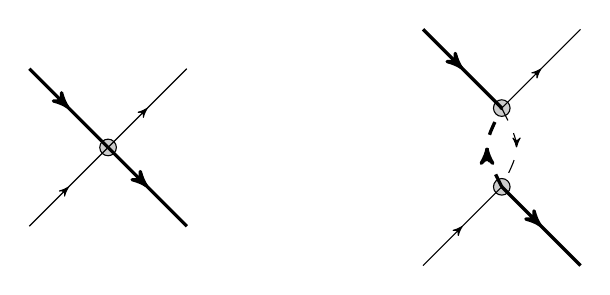
\begin{tikzpicture}
\node at (0,0) [graphnode]{};
\draw [->-, very thick] (-1,1) to node[above]{} (0,0);
\draw [->-, very thick] (0,0) to node[below]{} (1,-1);
\draw [->-] (-1,-1) to node[below]{} (0,0);
\draw [->-] (0,0) to node[above]{} (1,1);

\node at (5,0.5) [graphnode]{};
\node at (5,-0.5) [graphnode]{};
\draw [->-, very thick] (4,1.5) to node[above]{} (5,0.5);
\draw [->-, very thick] (5,-0.5) to node[below]{\hspace{2cm}} (6,-1.5);
\draw [->-] (4,-1.5) to node[below]{} (5,-0.5);
\draw [->-] (5,0.5) to node[above]{} (6,1.5);

\draw [dash pattern=on5pt][->-, very thick] (5,-0.5) .. controls (4.75,0) .. (5, 0.5) node[pos=0.5,left] {};
\draw [dash pattern=on5pt][->-] (5,0.5) .. controls (5.25,0) .. (5,-0.5) node[pos=0.5,right] {};

\end{tikzpicture}
\end{center}
\caption{ An illustration of the vertex splitting operation used for
	mapping  to .}
\label{fig:vertexsplit}
\end{figure}

\begin{fact}\label{fact:CorrectDeg}
Consider a digraph  that has a good decomposition, and consider
 such that
\textbf{(1)}~, \quad
\textbf{(2)}~for every dicycle , ,
	 is the same for all edges  of , and \quad
\textbf{(3)}~for every vertex  with indegree = 1 = outdegree,
.
Then, for the digraph  obtained by
applying the splitting operations, there exists
 such that
, and
.
\end{fact}
\begin{proof}
For each , we consider the dicycle .
Let  be the -value associated with the dicycle  of ,
i.e., .
Then, in  and ,
we fix , and
we fix .
It can be seen that  satisfies the given conditions.
\end{proof}


\begin{definition}
Consider the digraph .
For any , let .
\end{definition}


Thus 
consists of all the solid edges except those in  together with
all the dashed edges of .
Note that each vertex in  has exactly one incoming edge and
exactly one outgoing edge in . Thus  forms a set of
vertex-disjoint dicycles that partition .


\begin{definition}
\label{def:nicedigraph}
Let  be a digraph with indegree and outdegree 
at every vertex, and suppose that  has a good decomposition
with witness set .
Let  be the digraph obtained by applying splitting operations
to  and its good decomposition.
Then  is said to have the \textit{good tours} property if
 is connected
(i.e.,  forms a Hamiltonian dicycle of )
for each .
\end{definition}


{
\begin{figure}[htb]
\centering
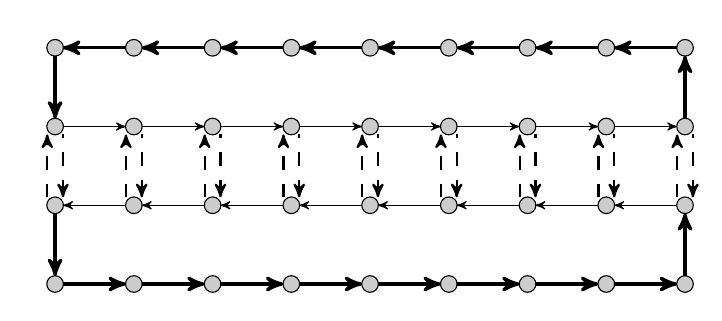
\begin{tikzpicture}
\foreach \x in {0,1,2,...,8}
{
	\node at (\x , 0) [graphnode]{};
	\node at (\x , 1) [graphnode]{};
	\node at (\x , 2) [graphnode]{};
	\node at (\x , 3) [graphnode]{};
}
\foreach \x in {0,1,2,...,7}
{
	\draw [->, very thick] (\x +0.1 , 0) to node[auto]{} (\x + 1-0.1 , 0);
	\draw [<-] (\x +0.1, 1) to node[auto]{} (\x + 1-0.1 , 1);
	\draw [->] (\x +0.1, 2) to node[auto]{} (\x + 1-0.1 , 2);
	\draw [<-, very thick] (\x +0.1, 3) to node[auto]{} (\x + 1-0.1 , 3);
}

\foreach \y in {0,2}
{
	\draw [<-, very thick] (0 , \y +0.1) to node[auto]{} (0 , \y +1-0.1);
	\draw [->, very thick] (8 , \y +0.1) to node[auto]{} (8 , \y +1-0.1);
}

\foreach \x in {0,1,2,...,7,8}
{
	\draw[dash pattern=on5pt] [->, thick] (\x -0.1 , 1+0.1) to node[auto]{} (\x -0.1, 2-0.1);
	\draw [dash pattern=on5pt][<-, thick] (\x +0.1, 1+0.1) to node[auto]{} (\x +0.1, 2-0.1);
}

\end{tikzpicture}
\caption{Digraph from Figure~\ref{fig-bal} after the splitting operation}
\label{fig-graph}
\end{figure}

\begin{figure}[htb]

\begin{center}
\subfloat[ ]{

\begin{tikzpicture}
\node at (0,0.5) [graphnode]{};
\node at (1,0.5) [graphnode]{};
\node at (3,0)[]{};
\node at (-2,1)[]{};
\draw [->-] (0 +0.1 , 0.5+0.1) .. controls(0 + 0.4, 0.75) .. node[auto]{} (0 + 1-0.1 , 0.5+0.1);
\draw [->-] (0 + 1-0.1 , 0.5-0.1) .. controls(0 + 0.4, 0.25) .. node[auto]{} (0 +0.1 , 0.5-0.1);
\end{tikzpicture}
}
\subfloat[ ]{
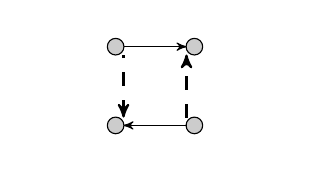
\begin{tikzpicture}
\node at (3,0) [graphnode]{};
\node at (3,1)[graphnode]{};
\node at (4,0)[graphnode]{};
\node at (4,1)[graphnode]{};
\draw [<-] (3 +0.1, 0) to node[below]{} (4 -0.1 , 0);
\draw [->] (3 +0.1, 1) to node[auto]{} (4 -0.1 , 1);
\draw[dash pattern=on5pt] [->, thick] (4 -0.1 , 0+0.1) to node[right]{} (4 -0.1, 1-0.1);
\draw [dash pattern=on5pt][<-, thick] (3 +0.1, 0+0.1) to node[auto]{} (3 +0.1, 1-0.1);
\node at (5,0)[]{};
\node at (2,0)[]{};
\end{tikzpicture}
}
\caption{ Transforming a dicycle  formed by
an anti-parallel pair of thin edges in Figure~\ref{fig-bal} to
 by the splitting operation.}
\label{fig-square}
\end{center}
\end{figure}



\begin{figure}[htb]
\centering
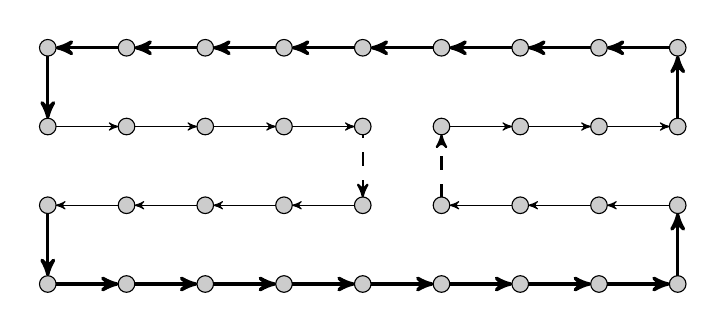
\begin{tikzpicture}
\foreach \x in {0,1,2,...,8}
{
	\node at (\x , 0) [graphnode]{};
	\node at (\x , 1) [graphnode]{};
	\node at (\x , 2) [graphnode]{};
	\node at (\x , 3) [graphnode]{};
}
\foreach \x in {0,1,2,...,7}
{
	\draw [->, very thick] (\x +0.1 , 0) to node[auto]{} (\x + 1-0.1 , 0);
	\draw [<-, very thick] (\x +0.1, 3) to node[auto]{} (\x + 1-0.1 , 3);
}
\foreach \x in {0,1,2,3,5,6,7}
{
	\draw [<-] (\x +0.1, 1) to node[auto]{} (\x + 1-0.1 , 1);
	\draw [->] (\x +0.1, 2) to node[auto]{} (\x + 1-0.1 , 2);
}
\foreach \y in {0,2}
{
	\draw [<-, very thick] (0 , \y +0.1) to node[auto]{} (0 , \y +1-0.1);
	\draw [->, very thick] (8 , \y +0.1) to node[auto]{} (8 , \y +1-0.1);
}
	\draw [dash pattern=on5pt] [<-, thick] (4 , 1 +0.1) to node[auto]{} (4 , 2-0.1);
	\draw [dash pattern=on5pt] [->, thick] (5 , 1 +0.1) to node[auto]{} (5 , 2-0.1);

\end{tikzpicture}
\caption{}
\label{fig-tour}
\end{figure}
}

\subsection{Certifying a feasible solution}

In what follows, we assume that  is a digraph
that satisfies the conditions stated in
Definition~\ref{def:nicedigraph}.
We focus on the digraph
 obtained by applying splitting operations to ;
observe that  depends on  as well as on
the given good decomposition of . Let  be the associated cone of .

Let  denote the set of images of the edges of  (the solid edges),
and let  denote the set of auxiliary edges (the dashed edges).
Given  and ,
let  denote the
set of indices  such that
 intersects ,
and let  denote the size of this set;
thus,  denotes the number of ``fractional cycles''
that intersect  in the solid edges.

Note that each (solid or dashed) edge  is in a unique cyle ;
let  denote the index of  in ;
if , then we use  to
denote .




Let  be a nonnegative integer.
We define the feasible solution  for
the level~ tightening of the DFJ-LP
(of ATSP, by the \iSA\ system)
as follows:
\begin{definition}\label{def:dfj-feasol}
For a nonnegative integer  and
for any subset  of ,
let  be a vector indexed by the elements of
 and defined as follows:
\label{def:dfj-zvec}

\end{definition}


Observe that the second case applies when
the set  has one or more dashed edges,
and moreover,  is contained in a
, ;
also, observe that there is at most one tour that contains ,
because the dashed edges are partitioned among the cycles ,
so each dashed edge in  belongs to a unique tour.


\begin{theorem}
\label{thm:dfj-feasible}
Let  be a strongly connected digraph that
has a good decomposition with witness set~,
and moreover,
has (i)~both indegree and outdegree  for every vertex,
and (ii)~satisfies the ``good tours'' property.
Then, for any nonnegative integer , and
any  with ,
we have

\end{theorem}

\begin{proof}
Note that  by Definition~\ref{def:dfj-feasol}.
Thus, we only need to prove .
The proof is by induction on .
The base case is important, and it follows easily from the
good decomposition property and the ``good tours'' property of .
This is done in Lemma~\ref{lemma:dfj-basecase} below, where we show that
.

In the induction step, we assume that
 for some integer 
(the induction hypothesis),
and we apply the recursive definition based
on the shift operator, namely,
 iff for each 

Lemma~\ref{lemma:dfj-cond1} (below) proves (\ref{eq:dfj-cond1}) and
Lemma~\ref{lemma:dfj-cond2} (below) proves (\ref{eq:dfj-cond2}).
\end{proof}

The next lemma proves the base case for the induction;
it follows from the ``good tours'' property of the digraph.

\begin{lemma} \label{lemma:dfj-basecase}

\end{lemma}

\begin{proof}
Note that .
Let  be the subvector of 
on the singleton sets .
We need to prove that  is a feasible
solution of the DFJ~LP.
It can be seen that  is as follows:
if , then ,
otherwise, if  ( is a solid edge), then ,
otherwise, if  ( is a dashed edge), then .
Clearly,  is in  and satisfies the degree constraints.
Now, we need to verify that  satisfies the cut constraints
in the digraph .
Consider any nonempty set of vertices , and the cut .

Observe that , hence, there are at least two indices
 such that .
Hence, both  and  exist;
moreover, every edge  (either solid or dashed) in either
 or  has .
Clearly, each of  and  has
at least one edge in .
Let  be an edge of  that is in .
If , then we are done,
since we have .
Thus, we may assume .
Now, we have two cases.

First, suppose that  is a dashed edge.
Then, note that the edge of  in ,
call it , is distinct from 
(since the tours are disjoint on the dashed edges),
and again we are done, since .

In the remaining case,  is a solid edge
and .
Then, , and so 

exists and it has at least one edge  in ;
moreover,  because 

contains none of the solid edges of the cycle .
Thus, we are done, since .
It follows that  staisfies all of the cut constraints.

\end{proof}


The following fact summarizes some easy observations;
this fact is  used in the next lemma.

\begin{fact}
\label{fact:set-intour}
Let  be a subset of .
Suppose that  is not contained in any
, .
\textbf{(1)}
Then, for any edge ,
 is also not contained in any
, .
\textbf{(2)}
Similary, for any index ,
 is not contained in any
, .
\end{fact}



\begin{lemma}
\label{lemma:dfj-cond1}
Suppose that for any nonnegative integer  and
any  with ,
we have . Then for any  with ,

\end{lemma}

\begin{proof}
For any edge  and any ,
the definition of the shift operator gives


Let  denote the cycle containing edge ,
and let  denote the index of  in .

We will show that

Lemma \ref{lemma:dfj-recursive} (below) shows that

Hence, for every edge  (i.e., in every case),  is in .
\begin{description}{
\item[Case~1.]

{( is a solid, integral edge)}.
We apply Definition~\ref{def:dfj-zvec} (the definition of ), and
consider the three cases in it:
\\
\begin{description}{
\item[Subcase~1.1.]
.
Then we have , and moreover,
we have 
(the number of ``fractional cycles'' intersecting  and 
is the same, since  is a non-fractional edge).
Hence, .
\\
\item[Subcase~1.2.]
 and
.
Then it is clear that  and ,
because  contains every solid edge except those in
the fractional cycle .
Hence, .
\\
\item[Subase~1.3.]
 and
.
Then it is easily seen that both conditions apply to  (rather than ).
Hence, .
}\end{description}

\item[Case~2.]
We have

{( is a dashed, integral edge)}.
We apply Definition~\ref{def:dfj-zvec}, noting that
 and
there exists no index  such that 
(no ``valid tour'' contains a dashed, integral edge),
hence, .

\item[Case~3.]
We have

{( is a solid, fractional edge)}.
We apply Definition~\ref{def:dfj-zvec}.
We have two subcases, either
, or not.
\\
\begin{description}{
\item[Subcase~3.1.]
If , then .
Thus, the analysis is the same as in the previous section; in particular,
see Equation~\eqref{eqn:bal-case1} in the proof of Lemma~\ref{lemma:cond1}.
Hence, we have
.

\item[Subcase~3.2.]
Otherwise, .
Then we have two further subcases:
either there is an  with 
or not.
\\
\begin{description}{
\item[Subcase~3.2.1]
Consider the first subcase;
thus,  where .
Note that  is not contained
in other tours since .
We have two further subcases, either  or not.

\begin{description}{
\item[Subcase~3.2.1.1.]
If , then ,
hence, 
(by the last case in the definition of );
moreover, note that  is the unique tour containing 
but it is \emph{not} a ``valid tour'' w.r.t.\ ,
hence, 
(by the last case in Definition~\ref{def:dfj-zvec}).

\item[Subcase~3.2.1.2.]
Otherwise, if , then
, and moreover,
 \emph{is} a ``valid tour'' w.r.t.\ 
(since  and ),
hence, we have

(by the second case in Definition~\ref{def:dfj-zvec},
for both LHS and RHS).
}\end{description}

\item[Subcase~3.2.2.]
Consider the last subcase;
thus,  for all .
Then by Fact~\ref{fact:set-intour}, the same assertion
holds w.r.t.\  (rather than ),
as well as w.r.t.\  (rather than ).
Hence, we have

(by the last case in Definition~\ref{def:dfj-zvec},
for both LHS and RHS).
}\end{description}
} \end{description}

\item[Case~4.]
We have

{( is a dashed, fractional edge)}.
We apply Definition~\ref{def:dfj-zvec}, noting that
.
We have two subcases, either
, or not.
If , then the second case of
Definition~\ref{def:dfj-zvec}
together with the fourth case of Equation~\eqref{eqn:dfj-case1}
(the definition of ) gives
.
Otherwise, , and then we have
;
note that the last case of Definition~\ref{def:dfj-zvec}
applies because  is
the unique ``valid tour'' that could contain .
}\end{description}
\end{proof}


Lemma~\ref{lemma:dfj-recursive} shows that ,
restricted to ,
is in ;
this is used in Lemma~\ref{lemma:dfj-cond1} to show that 
is in .


\begin{lemma}
\label{lemma:dfj-recursive}
For any nonnegative integer ,
any ,
any  with ,
and any ,
we have

\end{lemma}
\begin{proof}
We have .

We apply Definition~\ref{def:dfj-zvec} (the definition of )
to , and we have three cases.

\begin{description}{
\item[Case~1.]
.
Then .
For the RHS, we have two subcases, either  or not.
In the first subcase, we have 
(since  contains none of the solid edges of ),
hence, ,
consequently, the RHS is
,
which is the same as the LHS.
In the other subcase, .
Then, we have 
(because  and  contains all solid edges
except those in ), hence,
,
and consequently, the RHS is
,
which is the same as the LHS.

\item[Case~2.]
 and
there exists  such that .
Then ,
by Definition~\ref{def:dfj-zvec}.
For the RHS, we have two subcases, either  or not.
In the first subcase, we have ,
because  is the unique tour containing 
but it is \emph{not} a ``valid tour'' w.r.t.\ ,
hence, the last case in Definition~\ref{def:dfj-zvec} applies.
Thus, the RHS is
,
which is the same as the LHS.
In the second subcase, .
Then, in the RHS, ,
because  and 
so the second case in Definition~\ref{def:dfj-zvec} applies.
Moreover, ,
because , and  is the unique tour containing ,
so .
Thus, the RHS is
,
which is the same as the LHS.

\item[Case~3.]
 and
, .
Then .
In the RHS, ,
by the third case in Definition~\ref{def:dfj-zvec},
since the relevant conditions hold (by Fact~\ref{fact:set-intour}).
Moreover, ,
because  and .
Thus, the RHS is
,
which is the same as the LHS.
}\end{description}
This completes the proof of the lemma.
\end{proof}


\begin{lemma}
\label{lemma:dfj-cond2}
Suppose that for any nonnegative integer  and
any  with ,
we have . Then for any  with ,

\end{lemma}
\begin{proof}By Lemma~\ref{lemma:dfj-cond1} and
Lemma~\ref{lemma:dfj-recursive}, we have for each  and
any ,

Hence, in every case, 
\end{proof}


\begin{theorem}\label{thm:dfj-sgIR}
Let  be a nonnegative integer, and let 
satisfy .
There exists a digraph on  vertices
such that the integrality ratio for
the level~ tightening of the standard~LP (DFJ~LP)
(for ATSP, by the \sa\ procedure)
is .
\end{theorem}

\begin{proof}
Given  and , we
fix  to get a digraph  shown in
Figure~\ref{fig-bal} where  is the length of the ``middle path''.
Let the cost of each  edge in  be~.
Then we construct  from .
We keep the cost of edges in  to be~ and fix
the cost of new edges to be~.
See Figure~\ref{fig-graph}; each solid edge has cost~ and
each dashed edge has cost~.
In the proof of Theorem \ref{thm:sgbalIR}, we claimed that
the minimum cost of an Eulerian subdigraph of  is .
It can be seen that the minimum cost of an Eulerian subdigraph of
 is .
(To see this, take an Eulerian subdigraph of ,
then contract all dashed edges contained in it,
to get an Eulerian subdigraph of  of the same cost.)
Let  be the metric completion of .
Then, the optimal value of the integral solution in
 is .

Now we invoke Theorem~\ref{thm:dfj-feasible}, according to which
the fractional solution 
(Definition \ref{def:dfj-feasol}) is in ;
see Figure~\ref{fig-graph};
we have
 for each solid, thick edge 
(the solid edges of the outer cycle),
 for each solid, thin edge 
(the solid edges of the middle paths), 
while the value of the dashed edges do not contribute to the value of the objective.
By Section \ref{sec:EVto0}, this feasible solution can
be extended to a feasible solution in .



Hence, the integrality ratio of  is

\end{proof}






\section{Path ATSP}

Let  be a digraph with nonnegative edge costs , and let 
and  be two distinguished vertices. We define
 to be the polytope of the following LP that has a variable  for each edge  of :




In particular, when  is a complete digraph with metric costs, the
above LP is the standard relaxation
for the - path~ATSP, which is to compute a Hamiltonian (or,
spanning) dipath from  to  with minimum cost in the complete
digraph with metric costs. For  , we denote the
associated cone by .

(In the literature, the notation for the two distinguished vertices is
, but we use  to avoid conflict with our symbol  for the
number of rounds of the \iSA\ procedure.)

An \textit{-Eulerian subdigraph}  of  is  together
with a collection of edges of  with multiplicities such that (i) for
any , the indegree of  equals its outdegree and
(ii) the outdegree of  is larger than its indegree by  and the
indegree of  is larger than its outdegree by  and (iii) 
is weakly connected (i.e., the underlying undirected graph is
connected). The - path~ATSP on the metric completion  of 
is equivalent to finding a minimum cost -Eulerian subdigraph of
.


For any subset  of , we use  to denote
the subdigraph of  induced by . As before, we use  to denote  (for the groundset ). Also, by the \emph{restriction} of  on  we mean the vector
 that
is given by

for all .



\begin{lemma}
\label{reduction}
Let  be a nonnegative integer.
Let .
Suppose that there exists a dipath 
from some vertex  to another vertex 
such that
 for each .
Let  denote the set of internal vertices of the dipath , and
let .
Then,

\end{lemma}

\begin{proof}
Let  and let
, i.e., .
The proof is by induction on .
Denote  by  for short.
Clearly, .
Thus, we only need to prove
.

\noindent \textbf{Base case:}
.
Let  be the subvector of  on the singleton sets
, and let  be the subvector of
 on the singleton sets.

We have to prove that  is a feasible solution of
. It is easy to see that
 is in  and it satisfies the
degree~constraints. Thus, we are left with the verification of the cut
constraints.  Observe that each positive edge (on which  is
positive) of  with its head (tail) in  has its tail (head) in
 ().
Let .
If , then
observe that every edge in  has
its head in , hence, we have
.
Similarly, if , then we have
;
the equation holds because every edge in  has
its tail in .

\noindent \textbf{Induction Step:}
For , we know

if and only if for any ,


Since  is a feasible solution in , we
have


Note that . For any  such that
, we have . Thus,
.
Similarly, we have  .
For any , since , we have
 (by the definition of the \iSA\ procedure),
hence, we have

Similarly,

\noindent \textbf{Case 1:} .
In this case, all items in  are zero. This implies .

\noindent \textbf{Case 2:} .
In this case, we consider . Note that
 for any  and
 with value 
at the item indexed by .
By the inductive hypothesis, we have
, i.e.,
. Thus, .
\\
Similarly, we have . This completes the proof.
\end{proof}

From the last section, we know that 
(Definition~\ref{def:dfj-feasol}) is in
, where  is defined in
Figure~\ref{fig-graph};
note that  is obtained from the
digraph and the good decomposition given in Figure~\ref{fig-bal}.
The solid edges in  have cost~ and the
dashed edges in  have cost~.

Let  be the right-most vertex in the second row
	(incident to two dashed edges),
let  be the  left-most vertex in the second row
	(incident to two dashed edges),
and let  be the dipath of solid edges from  to .
By the definition of , we have
 for each . Let
 where  where
 is the set of internal vertices of the dipath . The next
result is a direct corollary of Lemma~\ref{reduction}.

\begin{corollary}\label{thm:PATSP-feasol}
We have 

\end{corollary}

The proof of the next lemma follows from arguments similar to
those in the proof of Theorem \ref{thm:dfj-sgIR}.
\begin{lemma}\label{PATSP:is-lowerbound}
The minimum cost of a -Eulerian subdigraph of  is
, where  is the number of edges in
the middle path in .
\end{lemma}

\begin{theorem}
Let  be a nonnegative integer, and let 
satisfy .
There exists a digraph on  vertices
such that the integrality ratio for
the level~ tightening of  by the \sa\ procedure is
.
\end{theorem}
\begin{proof}
Given  and , we
fix .
Consider the metric completion  of . By Section
\ref{sec:EVto0}, we can extend the feasible solution from 
Corollary~\ref{thm:PATSP-feasol} to a feasible solution to
. This gives an upper bound
on the optimal value of a fractional feasible solution to
. On the other hand,
Lemma \ref{PATSP:is-lowerbound} gives a lower bound on
the optimal value of an integral solution.
Thus, the integrality ratio is at least


\end{proof}



\paragraph {Acknowledgements:}
We thank a number of colleagues for useful discussions.
We are grateful to Sylvia Boyd and Paul Elliott-Magwood
for help with ATSP integrality gaps, and to
Levent Tun\c{c}el for sharing his knowledge of the area.





\bibliographystyle{abbrv}
\bibliography{atspbib}









\end{document}
